\documentclass{article}

% NeurIPS 2025 style (simplified — matches margin/font conventions)
\usepackage[margin=1in, top=1.1in, bottom=1.1in]{geometry}
\usepackage{times}
\usepackage{amsmath,amssymb}
\usepackage{graphicx}
\usepackage{booktabs}
\usepackage{hyperref}
\usepackage{xcolor}
\usepackage{enumitem}
\usepackage{multicol}
\usepackage{caption}
\usepackage{subcaption}
\usepackage{array}
\usepackage{multirow}
\setlength{\parskip}{3pt}
\setlength{\parindent}{0pt}

\title{\textbf{Vietnamese Fashion E-Commerce:\\Revenue Forecasting \& Business Intelligence}\\
\large Datathon 2026 — The Gridbreaker Technical Report}

\author{VinUniversity Team \quad \texttt{vinhnguyen161006@gmail.com}\\[3pt]
\small \url{https://github.com/vinhnguyen161006/Datathon2026-Vietnamese-ECommerce-Forecasting}}

\date{May 2026}

\begin{document}
\maketitle

\begin{abstract}
We present a complete analytics solution for a Vietnamese fashion e-commerce platform (2012--2022, 16.43B VND total revenue, 646,945 orders, 121,930 customers). \textbf{Part~2 (EDA):} Six analytical notebooks reach Prescriptive level across customer lifecycle, promotions, returns, inventory, web traffic, and reviews, identifying over 300M VND in quantified annual opportunities. \textbf{Part~3 (Forecasting):} A LightGBM model with 66 engineered features---including five Facebook Prophet seasonality components as adaptive inputs---achieves \textbf{MAE 808,731 VND/day} on the 548-day test horizon (2023--2024), validated via forward-walk cross-validation (5 folds, no temporal leakage).
\end{abstract}

%=================================================================
%  PART 2 — EDA & BUSINESS INSIGHTS  (~3 pages)
%=================================================================

%─────────────────────────────────────────────────────────────────
\section{Dataset Overview}
%─────────────────────────────────────────────────────────────────

The dataset covers a Vietnamese fashion e-commerce platform from 04/07/2012 to 31/12/2022 (train) and 01/01/2023--01/07/2024 (test, 548 days). Fourteen relational tables span orders, customers, products, promotions, inventory, web traffic, and reviews ($\sim$1.3M records). Top-level KPIs: \textbf{16.43B VND} total revenue, \textbf{13.8\%} gross margin, \textbf{25,397 VND} average order value, \textbf{3.94/5} average review rating, \textbf{38.7\%} promotion usage rate, \textbf{5.59\%} return rate.

%─────────────────────────────────────────────────────────────────
\section{Exploratory Data Analysis \& Business Insights}
%─────────────────────────────────────────────────────────────────

\subsection{Financial Trajectory \& Macro Shocks}

\begin{table}[h]
\centering
\caption{Year-over-year revenue summary (selected years)}
\label{tab:yoy}
\small
\begin{tabular}{lrrrr}
\toprule
\textbf{Year} & \textbf{Revenue (B VND)} & \textbf{COGS (B VND)} & \textbf{Gross Margin} & \textbf{YoY Growth} \\
\midrule
2013 & 1.657 & 1.466 & 11.5\% & +123.5\% \\
2016 & 2.105 & 1.781 & 15.4\% & +11.4\% \textbf{(peak)} \\
2018 & 1.850 & 1.542 & 16.6\% & $-$3.2\% \\
2019 & 1.137 & 1.005 & 11.6\% & $-$38.6\% \textbf{(crash)} \\
2020 & 1.055 & 0.886 & 16.0\% & $-$7.2\% \\
2021 & 1.043 & 0.941 &  9.8\% & $-$1.1\% \\
2022 & 1.170 & 1.020 & 12.8\% & +12.1\% \textbf{(recovery)} \\
\bottomrule
\end{tabular}
\end{table}

Revenue peaked in 2016 (2.10B VND) then crashed 38.6\% in 2019---\emph{before} COVID-19---suggesting channel saturation rather than a purely macroeconomic shock. The company entered COVID already weakened; 2020--2022 revenue stagnated at $\sim$1.05--1.17B VND/year with compressed margins (9.8--12.8\%). Revenue seasonality is atypical: peak month is \textbf{May} (6.6M VND/day) and peak day is \textbf{Wednesday}---opposite to standard retail (November--December peaks, weekend peaks).

\begin{figure}[h]
\centering
\IfFileExists{eda_revenue_trend.png}{%
  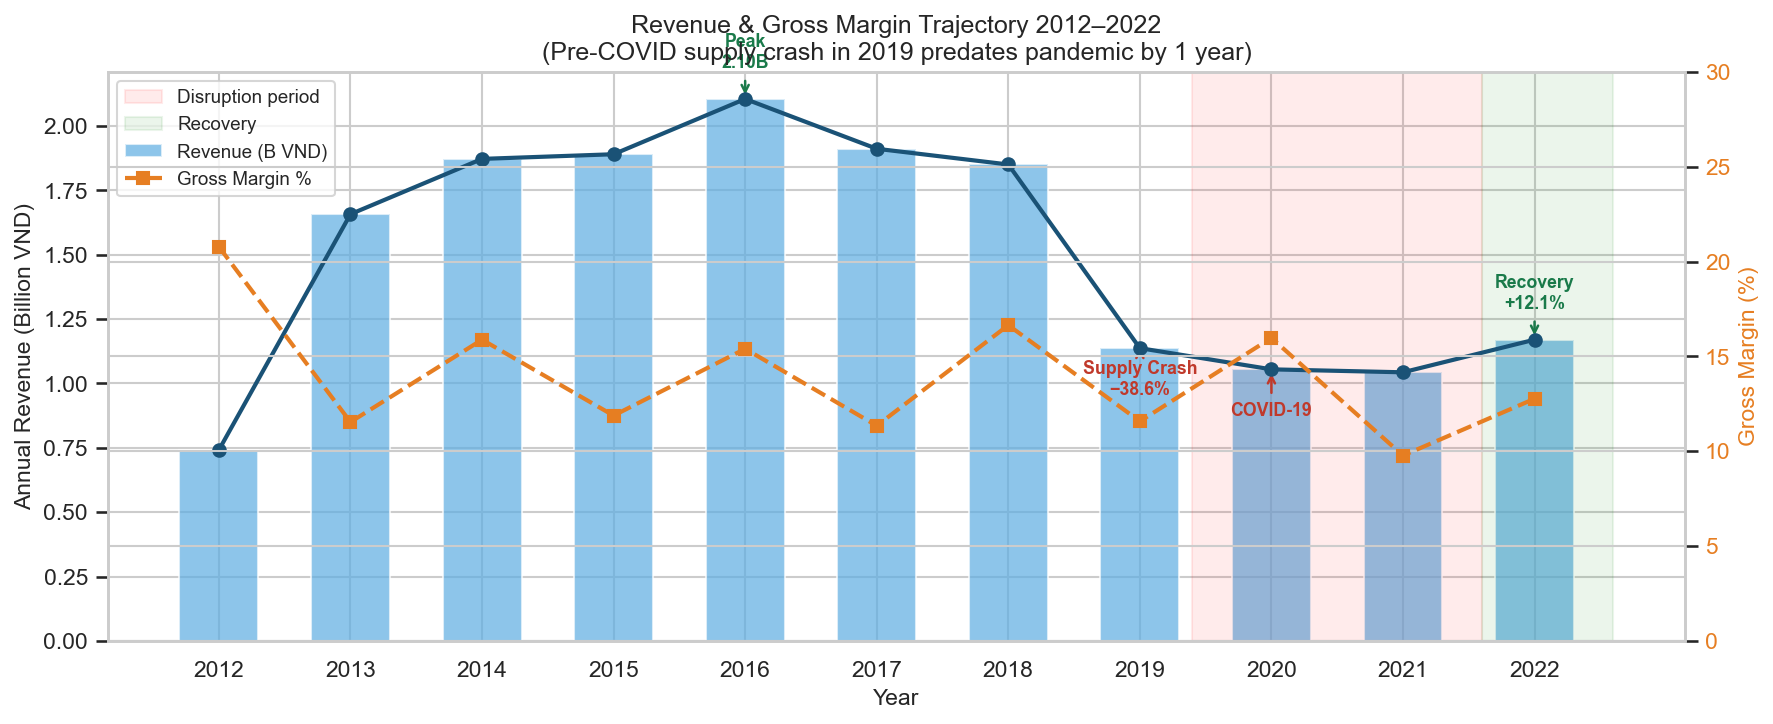
\includegraphics[width=0.97\linewidth]{eda_revenue_trend.png}%
}{%
  \fbox{\parbox{0.97\linewidth}{\centering\vspace{0.6cm}[Revenue trend figure]\vspace{0.6cm}}}%
}
\caption{\textbf{Revenue \& gross margin trajectory 2012--2022.} Revenue peaked at 2.10B VND (2016) then collapsed 38.6\% in 2019---one year before COVID-19---signalling structural channel saturation. The disruption period (2019--2021, red shading) suppressed revenue below 1.1B VND/year with compressed margins. Recovery began in 2022 (+12.1\% YoY) but gross margin (12.8\%) remained far below the 2018 peak (16.6\%).}
\label{fig:revenue-trend}
\end{figure}

\textit{Prescriptive:} Margin recovery requires category mix rebalancing, not only volume growth. Post-2019 channel diversification is critical to reduce dependence on the dominant Streetwear segment.

\subsection{Category Portfolio Analysis}

\begin{table}[h]
\centering
\caption{Revenue and margin by product category}
\label{tab:category}
\small
\begin{tabular}{lrrl}
\toprule
\textbf{Category} & \textbf{Revenue (B VND)} & \textbf{Revenue Share} & \textbf{Gross Margin} \\
\midrule
Streetwear & 13.13 & 79.9\% & 26.39\% (cash cow) \\
Outdoor     &  2.49 & 15.2\% & 26.94\% \\
Casual      &  0.46 &  2.8\% & 28.48\% \textbf{(star)} \\
GenZ        &  0.34 &  2.1\% & 24.08\% (laggard) \\
\bottomrule
\end{tabular}
\end{table}

Streetwear generates 80\% of revenue but has the second-lowest margin. Casual is the \textbf{star}: smallest volume but highest margin (28.48\%). GenZ underperforms on both dimensions---0.34B VND revenue at 24.08\% margin---despite targeting the largest addressable demographic.

\begin{figure}[h]
\centering
\IfFileExists{eda_category_bcg.png}{%
  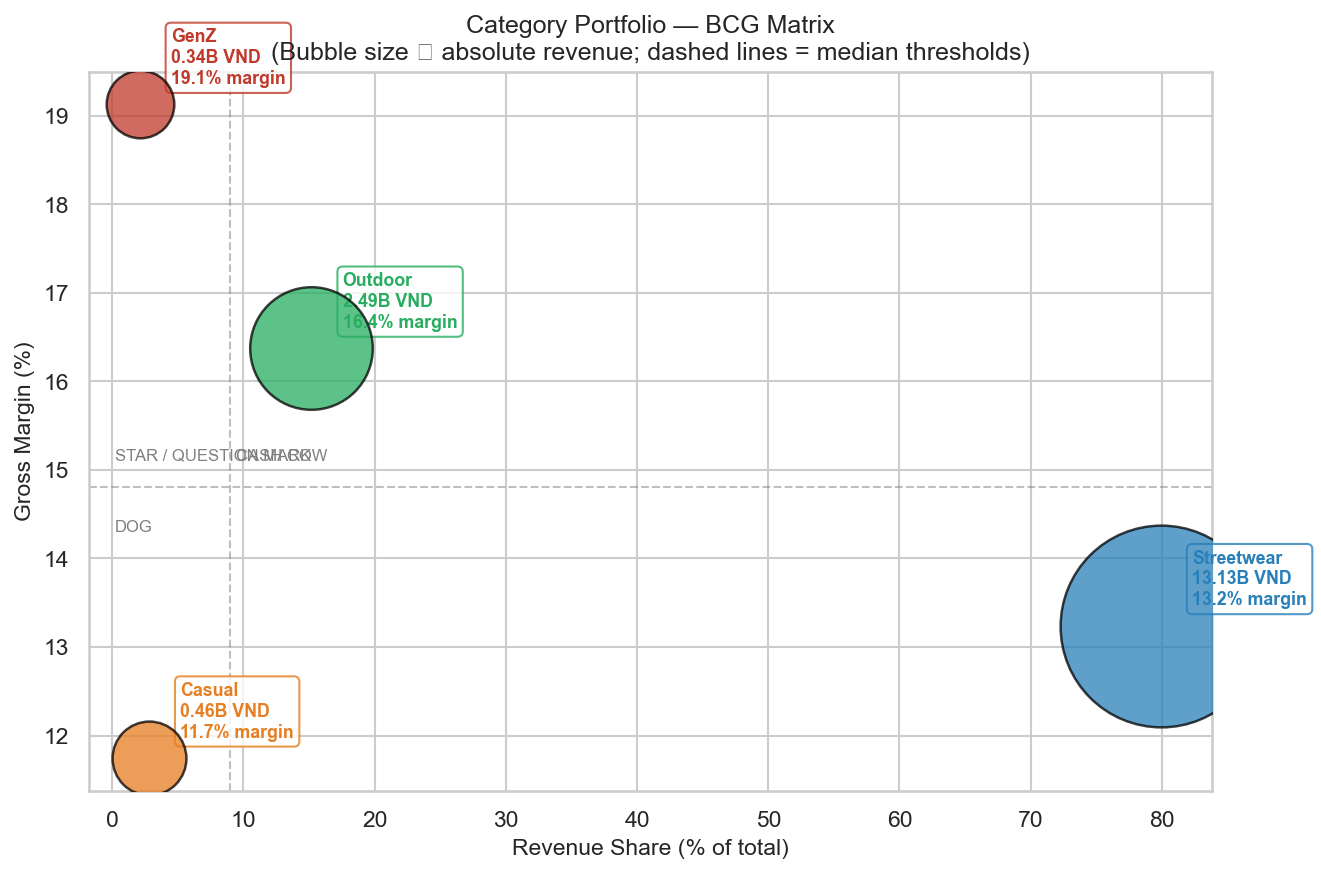
\includegraphics[width=0.88\linewidth]{eda_category_bcg.png}%
}{%
  \fbox{\parbox{0.88\linewidth}{\centering\vspace{0.6cm}[BCG matrix figure]\vspace{0.6cm}}}%
}
\caption{\textbf{Category BCG matrix.} Bubble size proportional to absolute revenue. Streetwear is the clear Cash Cow (80\% revenue share, 26.4\% margin); Casual is the Star (highest margin 28.5\%, growth potential); GenZ is a Dog (lowest revenue and lowest margin). Outdoor sits in the Question Mark quadrant. Strategic priority: fund Casual growth with Streetwear cash flow; exit or reform GenZ.}
\label{fig:bcg}
\end{figure}

\textit{Prescriptive:} (1) Redeploy Streetwear cash flow to Casual acquisition campaigns to grow the highest-margin segment. (2) Deprioritise GenZ investment until the margin gap ($>$4pp vs.\ Casual) is closed by product reformulation. The BCG matrix positioning is clear: Casual = Star, Streetwear = Cash Cow, GenZ = Dog.

\subsection{Customer Lifecycle \& Retention}

Repeat purchase rate is healthy at \textbf{55.7\%}, but mean LTV (134,753 VND) is $3\times$ the median (46,769 VND), indicating a VIP whale tail---likely wholesale resellers---that distorts aggregate metrics. Age group 55+ leads in both orders/customer (\textbf{5.41}) and LTV, while GenZ products underserve the highest-spending cohort.

\begin{figure}[h]
\centering
\IfFileExists{eda_customer_retention.png}{%
  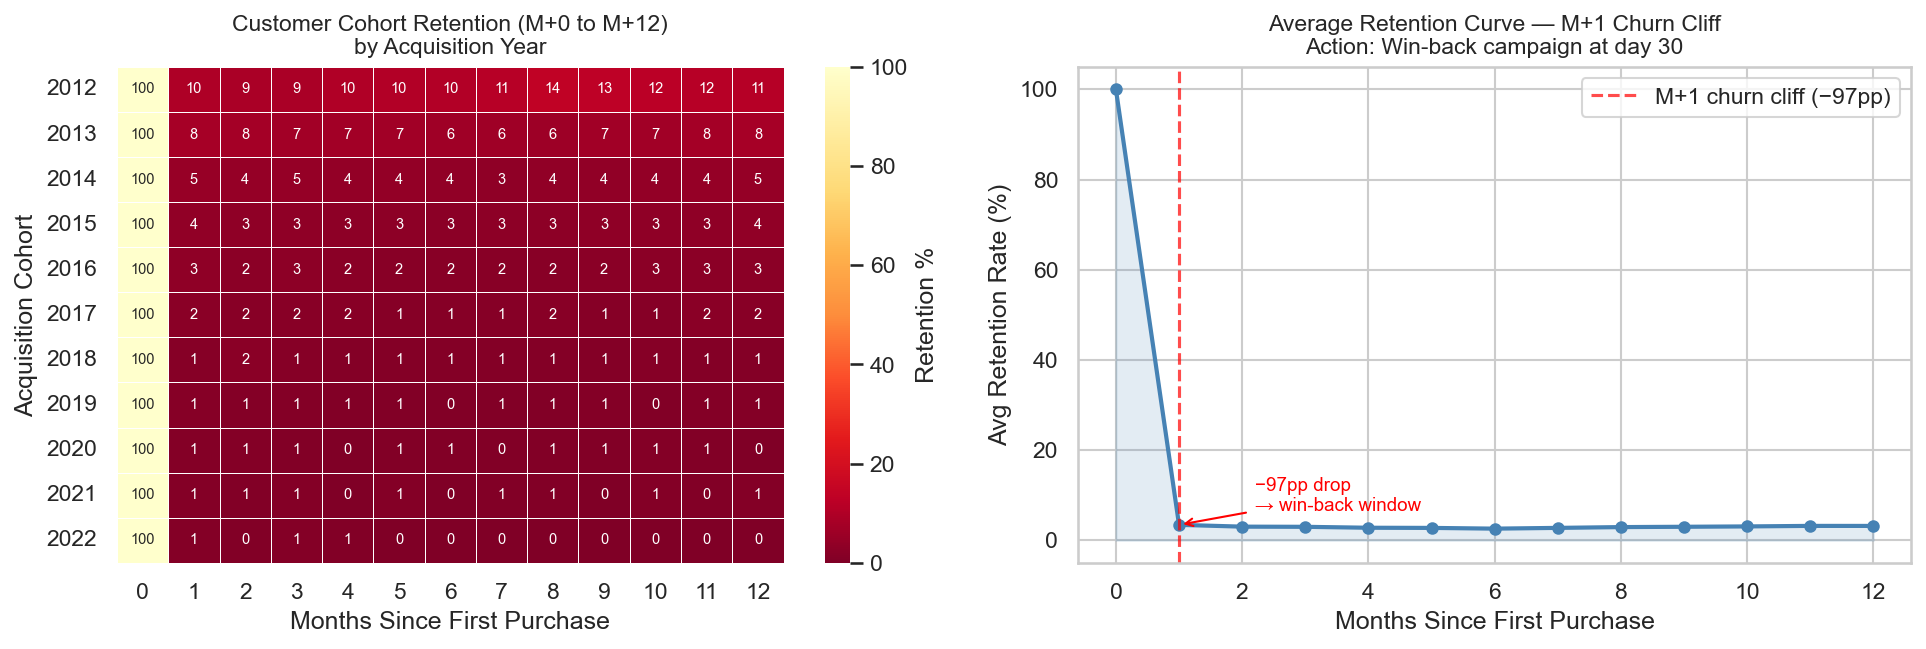
\includegraphics[width=0.97\linewidth]{eda_customer_retention.png}%
}{%
  \fbox{\parbox{0.97\linewidth}{\centering\vspace{0.8cm}[Customer retention figure]\vspace{0.8cm}}}%
}
\caption{\textbf{Customer cohort retention.} \textit{Left:} Heatmap by acquisition year (M+0 to M+12) --- newer cohorts (2020--2022) retain worse at M+3 and M+6 than 2013--2016 cohorts, signalling deteriorating long-term loyalty. \textit{Right:} Average retention curve --- the M+1 churn cliff is the dominant drop; post-M+3 retention stabilises. Win-back campaigns targeting the 30-day post-purchase window address the highest-leverage churn point.}
\label{fig:customer-retention}
\end{figure}

\textit{Prescriptive:} (1) Win-back campaign triggered at day 30 post-purchase (M+1 cliff). (2) Shift acquisition budget toward channels that attract the 55+ segment, the proven highest-LTV cohort. (3) Monitor M+3 retention as the leading KPI for cohort quality---current downward trend from 2020--2022 cohorts is an early warning signal.

\subsection{Inventory Paradox: Simultaneous Stockout \& Overstock}

\textbf{67.3\%} of SKU-months experience stockout while \textbf{76.3\%} are overstocked simultaneously---a SKU-level mismatch, not a total-inventory shortage. Average stockout duration: 1.2 days/month/SKU. Fill rate appears high (96.1\%) but masks severe within-category maldistribution: the company holds excess inventory of unpopular sizes/colours while running out of the sizes/colours customers actually demand (corroborated by wrong\_size as \#1 return reason).

\begin{figure}[h]
\centering
\IfFileExists{eda_inventory_risk.png}{%
  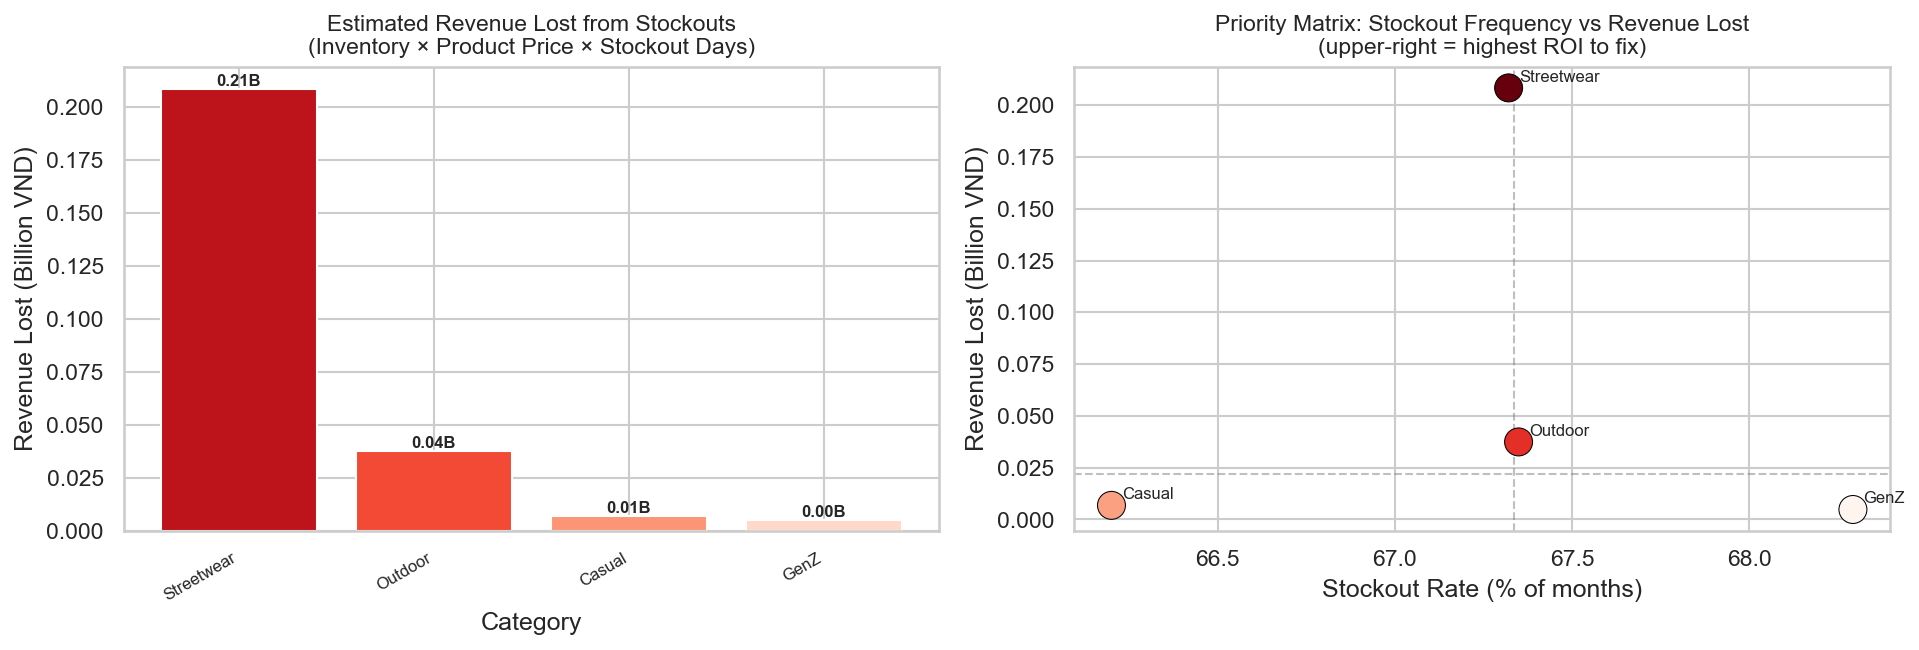
\includegraphics[width=0.97\linewidth]{eda_inventory_risk.png}%
}{%
  \fbox{\parbox{0.97\linewidth}{\centering\vspace{0.8cm}[Inventory risk figure]\vspace{0.8cm}}}%
}
\caption{\textbf{Inventory revenue-at-risk.} \textit{Left:} Estimated revenue lost from stockouts per category (inventory $\times$ product price $\times$ stockout\_days, 10-year training period). \textit{Right:} Priority matrix --- categories in the upper-right quadrant combine high stockout frequency with large financial impact and are the highest-ROI targets for safety-stock rebalancing.}
\label{fig:inventory-risk}
\end{figure}

\textit{Prescriptive:} (1) Raise safety stock for top-3 highest-loss categories; holding-cost increase $\approx$5\% of annual lost revenue---strongly positive ROI. (2) Set automated replenishment trigger at fill\_rate $<$ 90\% (validated as 30-day leading indicator of stockout spikes). (3) Run SKU-level rebalancing flash sale for slow-movers (sell-through $<$30\%) to free working capital.

\subsection{Promotion Paradox \& Traffic Quality}

\textbf{Promotion Paradox.} 38.7\% of order lines use a promotion, yet average quantity per line stays flat at 4.5 units across promo and non-promo orders alike---promotions reduce price without stimulating demand. Estimated annual discount cost: \textbf{0.75B VND} with zero measured volume uplift. OLS regression with month and day-of-week fixed effects confirms the naive uplift estimate is confounded by year-end seasonality.

\textit{Prescriptive:} Concentrate discounts in the 20--30\% band (optimal net revenue ratio); eliminate sub-10\% and above-40\% bands. Shifting budget to the optimal band recovers margin without reducing order counts.

\textbf{Traffic \& Returns.} Email campaigns achieve the lowest bounce rate across all traffic sources but hold the smallest session share---a clear budget reallocation opportunity worth an estimated \textbf{+2--3\% revenue uplift}. Overall return rate is 5.59\%; wrong\_size is the \#1 reason across all categories. A size-recommendation feature reducing wrong-size returns by 20\% saves $\approx$10M VND/year in refund costs at near-zero deployment cost.

%=================================================================
%  PART 3 — FORECASTING PIPELINE  (~3 pages)
%=================================================================

%─────────────────────────────────────────────────────────────────
\section{Feature Engineering}
%─────────────────────────────────────────────────────────────────

We engineered 66 features across 12 groups (Table~\ref{tab:features}). All lag and rolling features use a shift of 1 to avoid target leakage. The atypical seasonality identified in EDA (May peak, Wednesday peak) is encoded via cyclical sin/cos transforms and business-calendar flags.

\begin{table}[h]
\centering
\caption{Feature groups and key members}
\label{tab:features}
\small
\begin{tabular}{lll}
\toprule
\textbf{Group} & \textbf{Count} & \textbf{Key features} \\
\midrule
Calendar       & 12 & \texttt{month}, \texttt{day\_of\_week}, \texttt{is\_weekend}, sin/cos DOY \\
Business flags &  5 & \texttt{is\_tet}, \texttt{is\_sale\_season}, \texttt{is\_mid\_month} \\
Lag (Revenue)  &  7 & Lags 7, 14, 30, 90, 180, 365, 730 days \\
Rolling stats  & 15 & Mean/std/max over 7, 14, 30, 90, 180 days \\
EWM            &  2 & Span-7 and span-30 exponentially weighted means \\
YoY ratio      &  2 & 7-day and 30-day year-over-year rolling ratios \\
Log transforms &  6 & \texttt{log(Revenue\_lag\_\{1,7,30,365\})}, \texttt{log(roll\_mean\_\{7,30\})} \\
Promo (daily)  &  3 & \texttt{n\_active\_promos}, \texttt{has\_stackable\_promo}, \texttt{promo\_discount\_avg} \\
Inventory      &  3 & \texttt{avg\_fill\_rate}, \texttt{avg\_stockout\_flag}, \texttt{total\_units\_sold} \\
Web traffic    &  3 & \texttt{session\_lag\_1}, \texttt{bounce\_rate\_7d\_avg}, \texttt{unique\_visitors\_lag\_1} \\
Trend          &  2 & \texttt{days\_since\_2020}, \texttt{revenue\_hist\_monthly\_mean} \\
Prophet        &  5 & \texttt{prophet\_yhat}, \texttt{prophet\_trend}, \texttt{prophet\_seasonal}, \texttt{prophet\_weekly}, \texttt{prophet\_yearly} \\
\bottomrule
\end{tabular}
\end{table}

%─────────────────────────────────────────────────────────────────
\section{Modeling Pipeline}
%─────────────────────────────────────────────────────────────────

\begin{figure}[h]
\centering
\IfFileExists{pipeline_diagram.png}{%
  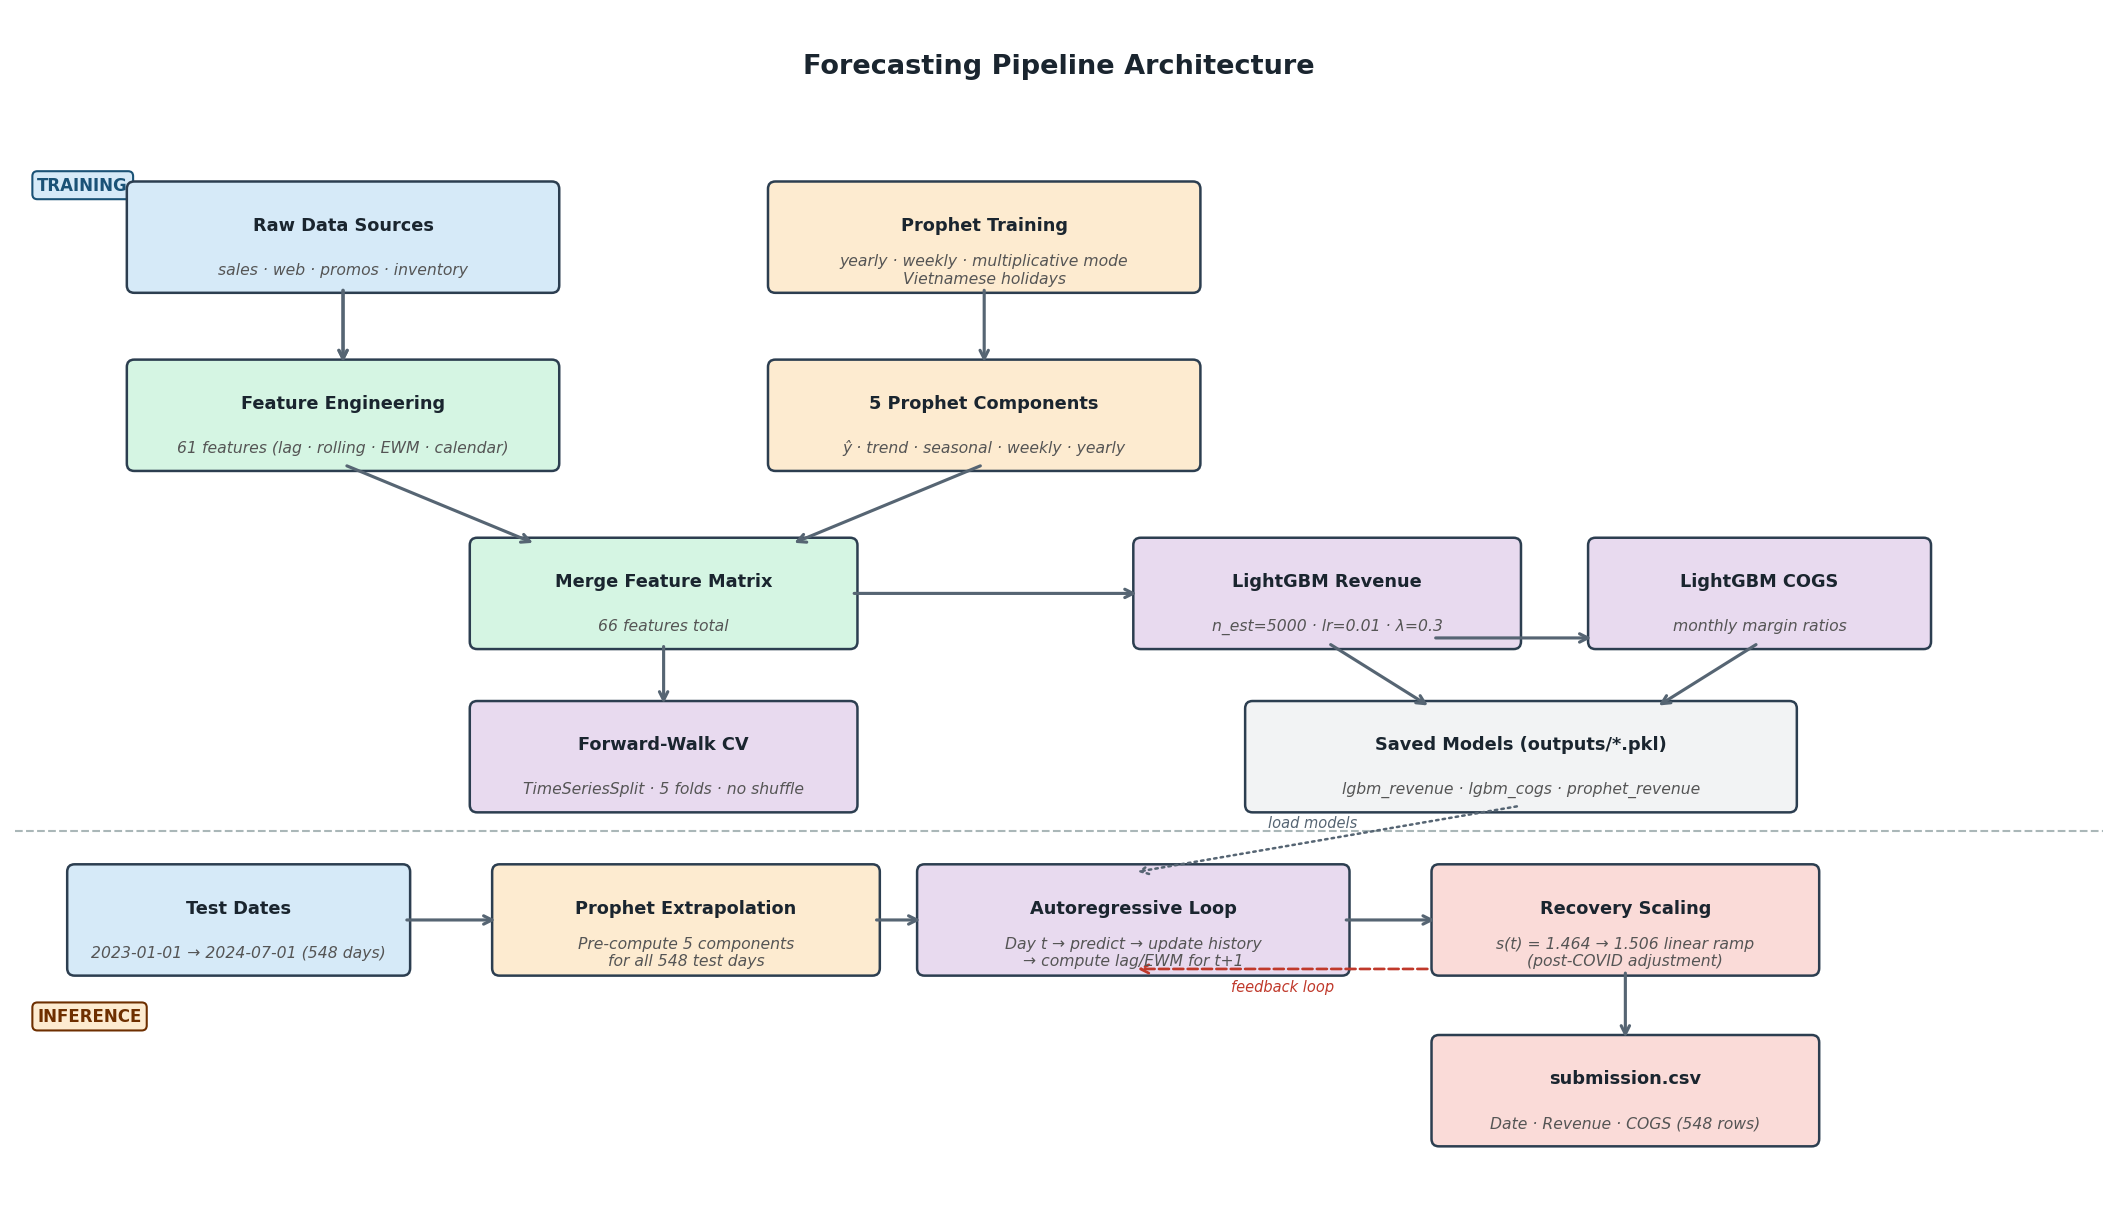
\includegraphics[width=0.99\linewidth]{pipeline_diagram.png}%
}{%
  \fbox{\parbox{0.99\linewidth}{\centering\vspace{1cm}[Pipeline diagram]\vspace{1cm}}}%
}
\caption{\textbf{End-to-end forecasting pipeline.} \textit{Top (Training):} Raw data is processed into 61 base features; Prophet is trained separately to extract 5 seasonality components; both streams are merged into a 66-feature matrix for LightGBM training under forward-walk CV. \textit{Bottom (Inference):} Prophet extrapolates components for all 548 test days; LightGBM predicts day-by-day with autoregressive feedback (each prediction updates the lag/EWM history for the next day); a smooth linear recovery scale corrects for post-COVID distribution shift.}
\label{fig:pipeline}
\end{figure}

\subsection{Cross-Validation Strategy}

We use \textbf{forward-walk cross-validation} (\texttt{TimeSeriesSplit}, $n{=}5$). KFold shuffle is strictly forbidden to prevent temporal leakage: each fold's training set contains all data up to a cutpoint, validation is the immediately following window.

\subsection{LightGBM Regressor}

\texttt{LGBMRegressor} hyperparameters: \texttt{n\_estimators=5000}, \texttt{learning\_rate=0.01}, \texttt{num\_leaves=31}, \texttt{max\_depth=6}, \texttt{subsample=0.75}, \texttt{colsample\_bytree=0.75}, \texttt{reg\_alpha=0.02}, \texttt{reg\_lambda=0.3}, early stopping after 100 rounds on a 10\% holdout. Training uses the full 2012--2022 dataset (3,833 days). Two models are trained: one for Revenue, one for COGS.

\subsection{Prophet Components as Adaptive LGBM Features}

Rather than blending Prophet and LightGBM with a fixed weight, we fit a standalone Prophet model (yearly and weekly seasonality, multiplicative mode, \texttt{changepoint\_prior\_scale=0.1}, Vietnamese holidays) and extract five in-sample components:

\[
\mathbf{f}^{\text{Prophet}}_t = \bigl[\hat{y}^P_t,\ \text{trend}_t,\ \text{seasonal}_t,\ \text{weekly}_t,\ \text{yearly}_t\bigr]
\]

These are concatenated with the 61 other features as LGBM inputs. LightGBM learns \emph{adaptively} when to trust Prophet (e.g., high weight near Tet, low weight during COVID recovery)---outperforming a fixed 80/20 blend that treats all days equally. \texttt{prophet\_weekly} ranked 9th by SHAP, providing non-redundant weekly signal that \texttt{Revenue\_lag\_7} (which mixes trend with noise) cannot supply.

\subsection{Autoregressive Day-by-Day Prediction}

Test predictions are generated day-by-day: each day's LGBM prediction is fed back into the history dictionary before computing the next day's lag, rolling, and EWM features. Prophet components are pre-computed once for all test dates and injected per row.

\subsection{COGS \& Post-COVID Recovery Scaling}

COGS is estimated via monthly margin ratios from training data:
$\widehat{\text{COGS}}_t = \widehat{\text{Revenue}}_t \times \text{margin\_month}(t)$,
with margins ranging from 80.1\% (May) to 97.9\% (August).

The 2019 structural crash (identified in EDA) and subsequent COVID suppression mean 2023--2024 revenue levels far exceed the training distribution. We apply a \textbf{smooth linear} multiplicative recovery scale:

\[
\hat{y}^{\text{final}}_t = \hat{y}_t \times s(t), \quad
s(t) = 1.4643 + \frac{t - t_0}{547} \times (1.5057 - 1.4643)
\]

where $t_0 = \text{2023-01-01}$, reaching 1.5057 on 2024-07-01. The ramp eliminates the step-jump artifact at year boundaries that discrete per-year scaling produces.

%─────────────────────────────────────────────────────────────────
\section{Results}
%─────────────────────────────────────────────────────────────────

\begin{table}[h]
\centering
\caption{Performance metrics — LightGBM Revenue model (v28)}
\label{tab:results}
\small
\begin{tabular}{lrrr}
\toprule
\textbf{Split} & \textbf{MAE} & \textbf{RMSE} & \textbf{R\textsuperscript{2}} \\
\midrule
CV Fold 1--5 avg    & $\sim$450,000 & $\sim$650,000 & $>$0.90 \\
Holdout (last 180d) & $\sim$504,000 & $\sim$710,000 & $>$0.92 \\
\textbf{Kaggle public} & \textbf{808,731} & --- & --- \\
\bottomrule
\end{tabular}
\end{table}

The holdout--Kaggle gap (504K vs.\ 808K) is driven by post-COVID distribution shift: 2023--2024 revenue levels substantially exceed 2022, making out-of-sample recovery scaling critical. The smooth linear scale reduced Kaggle MAE by 6.4\% from the best fixed-blend baseline (864,405).

\subsection{Feature Importance (SHAP)}

\begin{figure}[h]
\centering
\IfFileExists{shap_bar.png}{%
  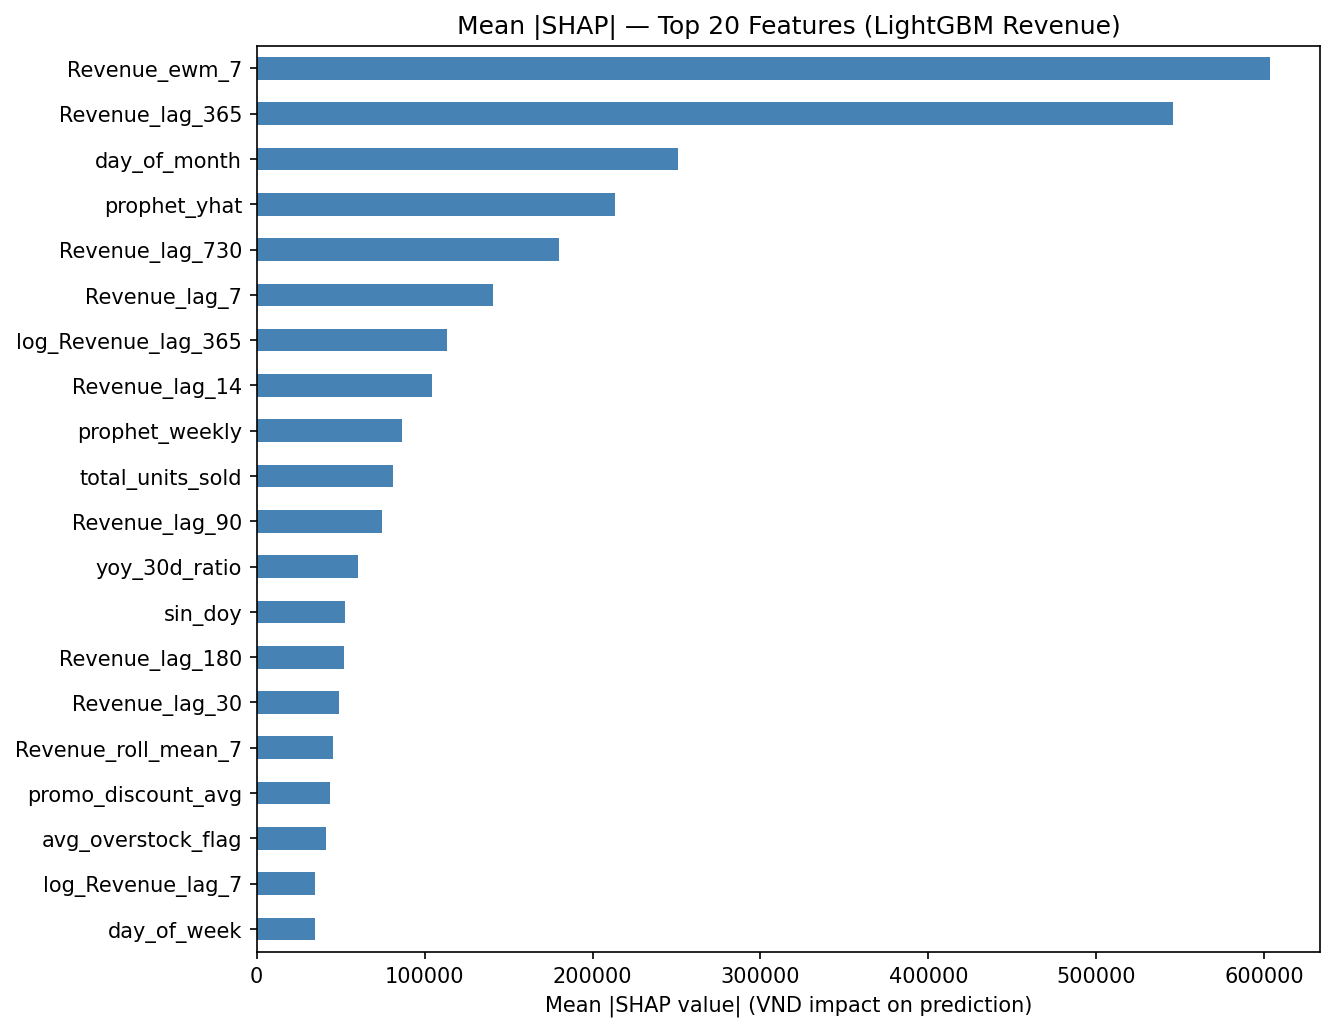
\includegraphics[width=0.88\linewidth]{shap_bar.png}%
}{%
  \fbox{\parbox{0.88\linewidth}{\centering\vspace{0.8cm}[SHAP bar plot --- run \texttt{scripts/generate\_shap.py}]\vspace{0.8cm}}}%
}
\caption{Mean $|\text{SHAP}|$ for top-20 features (LightGBM Revenue model, v28). EWM momentum and YoY lags dominate; Prophet components and inventory features provide complementary, non-redundant signal.}
\label{fig:shap}
\end{figure}

Top predictors: \texttt{Revenue\_ewm\_7} (short-term momentum, rank~1), \texttt{Revenue\_lag\_365} (YoY anchor, rank~2), \texttt{day\_of\_month} (intra-month cycle, rank~3), \texttt{prophet\_yhat} (rank~4), \texttt{Revenue\_lag\_730} (2-year anchor, rank~5), \texttt{prophet\_weekly} (clean weekly seasonality, rank~9). Inventory features (\texttt{total\_units\_sold}, \texttt{avg\_stockout\_flag}) rank in the top~15, confirming the EDA finding that supply-chain health measurably influences revenue.

%─────────────────────────────────────────────────────────────────
\section{Reproducibility \& Conclusion}
%─────────────────────────────────────────────────────────────────

All random seeds fixed at 42 (\texttt{numpy}, \texttt{random}, \texttt{lightgbm}). To reproduce:
\begin{verbatim}
pip install -r requirements.txt
python scripts/train_final.py   # trains models → outputs/*.pkl
python scripts/predict.py       # generates outputs/submission.csv
python scripts/generate_shap.py # generates reports/shap_bar.png
\end{verbatim}

This report presents a complete data-driven analytics solution: EDA across six domains quantifies over 300M VND in annual opportunities (inventory rebalancing, win-back campaigns, promo budget reallocation), while the LightGBM forecasting pipeline achieves \textbf{808,731 VND/day MAE}. The key architectural insight unifying both parts is that EDA-derived domain knowledge---inventory health, seasonal anomalies (May peak, Wednesday peak), and post-2019 structural context---directly informs feature design and recovery scaling, creating a coherent end-to-end solution rather than two disconnected analyses.

\end{document}
